%%%%%%%%%%%%%%%%%%%%%%%%%%%%%%%%%%%%%%%%%%%%%%%%%%%%%%%%%%%%%%%%%%%%%%%%%%%%%%%

\chapter{ANÁLISE E RESULTADOS}
\label{capanaliseseresults}

A possível natureza caótica da turbulência na camada limite atmosférica, no interior e acima da copa da floresta é investigada. Com base na aplicação de diversas ferramentas
%(já descritas no Capítulo~\ref{caputiltecnicas}) 
nas séries temporais em estudo, o objetivo deste trabalho é determinar se tais séries incluem componentes determinísticas que podem ser descritas (individualmente) por um sistema dinâmico de baixa dimensão, que se desenvolve em um atrator caótico.


\section{Estacionaridade}
Primeiramente, as séries temporais em estudo foram submetidas ao teste de estacionaridade.
% já descrito na Seção~\ref{subsecestacio}. 
A Tabela~\ref{tabelatempestacionaria} apresenta a classificação destas séries em estacionárias ou não estacionárias. Neste teste foram utilizadas janelas de dados deslizantes variáveis, a saber, $L=100,500$ e $1000$. Desta forma, as análises subseqüentes serão feitas apenas com as séries do tipo estacionárias.

\begin{table}[!ht]
\begin{center}
\caption{Análise da estacionaridade para as séries temporais de temperatura e velocidade do vento em diferentes períodos do dia e níveis da copa.}
\begin{tabular}{c c c}
\hline 
\textbf{Série temporal} & \textbf{Estacionaridade} \\
\hline
tS1200 & estacionária \\
tI1200 & estacionária \\
tS2300 & não-estacionária \\
tI2300 & estacionária \\
tM1200 & estacionária \\
wS1200 & estacionária \\
tM2300 & não-estacionária \\
\hline
\end{tabular}
\label{tabelatempestacionaria}
\end{center}
\end{table}

\section{Decomposição dos Dados}

Com o objetivo de investigar o papel das estruturas coerentes na existência (ou não) de caos na atmosfera, decidiu-se selecionar dentre o conjunto de séries disponíveis uma que apresentasse sinais nítidos da presença de estruturas coerentes em rampa e em seguida decompor a mesma (denominada de série total) em duas partes: uma parte dita coerente (baixas freqüências) e uma parte incoerente (altas freqüências). A parte coerente é caracterizada apenas pelas estruturas coerentes em rampa presentes na série total, enquanto que a parte incoerente é caracterizada pelas flutuações aparentemente aleatórias da mesma série. 

Desta forma, se a ocorrência de uma dinâmica de baixa dimensão na série temporal total estiver relacionada à presença de estruturas coerentes, é de se esperar que essa mesma dinâmica se manifeste também na série coerente, e que contrariamente, a série incoerente esteja associada à uma dinâmica de alta dimensão. Por inspeção visual, a série escolhida para as análises subseqüentes corresponde àquela que apresenta estruturas coerentes em rampa, a saber, a série de temperatura medida no nível superior da copa às 12 horas (tS1200), conforme a parte superior da Figura~\ref{figseriestempdiur}. 

%\subsection{Decomposição dos dados}

Inicialmente, a série temporal total (tS1200) foi decomposta em suas partes coerente e incoerente, por meio da filtragem com Wavelet de Haar~\cite{katul/94}, que é um tipo de ondeleta-mãe discreta, definida por

\begin{equation}
\left\{ \begin{array}{rrr} 1, &  & 0\leq t < 1/2 \\
                  -1, &  & 1/2\leq t < 1 \\
		   0, &  & \mbox{caso contrário}
\end{array} 
\right.
\label{eqwavelethaar}
\end{equation} 

% \begin{figure}[ht]
% \centering \resizebox{11cm}{!}{\includegraphics{Figuras/fighaar.pdf}}
% \caption{A wavelet de Haar, $\psi$}
% \label{fighaar}
% \end{figure}
Esta categoria de ondaletas é utilizada para detectar variações bruscas nos sinais, e trabalha com sinais temporais que tenham comprimentos da ordem da potência de dois mais próxima, ou seja, $2^{f}=s$, onde $s$ é o comprimento total da série, e $f$ é o número de freqüências possíveis para a decomposição. 

O comprimento da série em estudo é de $s=108.000$ pontos. Desta forma, não há um número exato de decomposições em freqüências, já que $f=16$ resulta em $s=65.536$ pontos e $f=17$ resulta em $s=131.072$ pontos. A estratégia utilizada foi completar o início da série temporal com zeros até que a freqüência $f=17$ fosse alcançada. 
 
Ainda não há na literatura um consenso de qual seja a melhor função ondeleta a ser utilizada para a decomposição e filtragem de uma série temporal. O que comumente se aceita é que a função ondeleta possua um formato característico próximo das características encontradas na série temporal. Isso explica o fato da Wavelet de Haar ter sido escolhida para a decomposição da série temporal de temperatura.  

A Figura~\ref{figfiltrotS0681200} mostra a série temporal total, a série temporal coerente (soma das baixas freqüências da série total) e a série temporal incoerente (soma das altas freqüências da série total), respectivamente. Após a filtragem da série total, $23072$ pontos iniciais foram descartados das séries total, coerente e incoerente; tal valor corresponde ao número de zeros inseridos na série total antes do procedimento de filtragem. É importante ressaltar que a soma da série coerente com a série incoerente resulta a série total, o que já era esperado.

\begin{figure}[ht]
\centering \resizebox{13cm}{!}{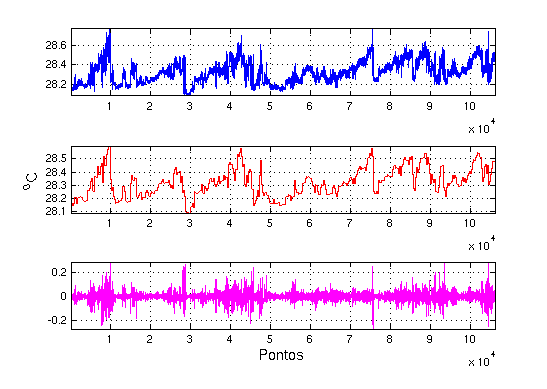
\includegraphics{Figuras2/filtrocoltS0681200.png}}
\caption{Sinal total (superior), soma das nove primeiras freqüências (meio), soma das sete últimas freqüências (inferior)}
\label{figfiltrotS0681200}
\end{figure}

\section{Caracterizando a turbulência acima da copa da floresta Amazônica}

O objetivo desta seção é verificar se as séries total, coerente e incoerente possuem as características típicas da turbulência plenamente desenvolvida, a saber, espectros de potência do tipo Kolmogorov e intermitência nas pequenas escalas. Aproveita-se para ilustrar o papel crucial das estruturas coerentes no transporte de propriedades (quantidade de movimento, calor, etc.) através da copa da floresta.

\subsection{Espectros de potência}

Os espectros de potência das séries temporais total, coerente e incoerente foram estimados usando FFT (ver Figura~\ref{figespectrotS0681200}). Os resultados mostram que as inclinações desses espectros no SI (em escala $\log$-$\log$) coincidem com a lei dos $-5/3$ de Kolmogorov. Esta observação demonstra que o fenômeno da turbulência está presente na série total, o que era esperado, mas também nas séries coerente e incoerente. Em especial, pode-se afirmar que a série incoerente está mais relacionada à turbulência de pequena escala do que a algum tipo de ruído. Este comportamento é consistente com outros estudos que utilizaram a mesma abordagem de separação de um fluxo turbulento em uma parte coerente e outra incoerente~\cite{farge/01}.


\begin{figure}[ht]
\centering \resizebox{15cm}{!}{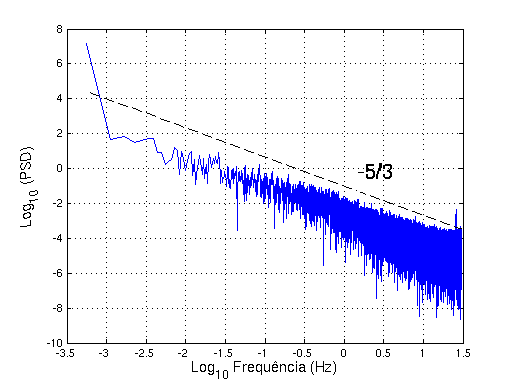
\includegraphics{Figuras2/tS0681200espectro.png}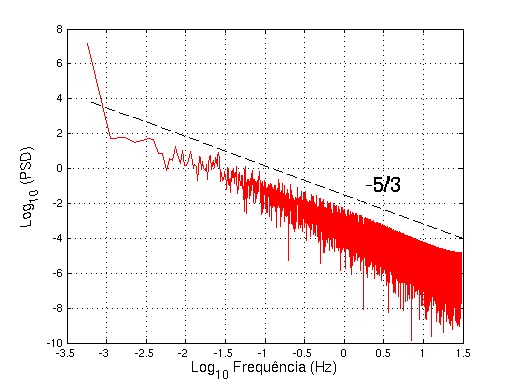
\includegraphics{Figuras2/ctS0681200espectro.png}}\\ \resizebox{7.5cm}{!}{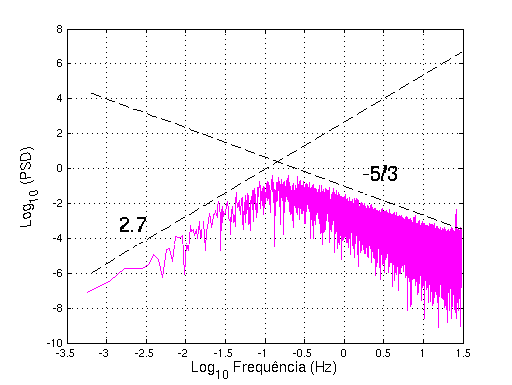
\includegraphics{Figuras2/itS0681200espectro.png}}
\caption{Espectros de potência da série temporal total (em azul), da série temporal coerente (em vermelho) e da série temporal incoerente (em rosa), respectivamente. Observe que as inclinações de todos os espectros no SI (em escala $\log$-$\log$) coincidem com a lei dos $-5/3$ de Kolmogorov. O espectro de potência associado a série incoerente possui uma inclinação adicional de $2.7$, que pode estar associada a um artefato numérico.}
\label{figespectrotS0681200}
\end{figure}

\subsection{Intermitência}

A detecção do fenômeno intermitente foi feita a partir das diferenças das séries de temperatura total, coerente e incoerente (medida às $12$ horas no nível superior) em várias escalas $r_{i}$ com $i=1,\ldots4$. Desta forma, as FDP's foram obtidas com base na distribuição estatística das diferenças $\Delta T_{r_{i}}=T(x+\Delta r_{i})-T(x)$. Os valores assumidos por $\Delta r_{i}$ são dados respectivamente por $1,10,100$ e $1000$, que para dados amostrados à $60$ Hz correspondem a $\Delta T_{t_{i}}$ de aproximadamente $0.0167,0.1667,1.6667$ e $16.6667$ segundos, respectivamente. A Figura~\ref{figintermitente} mostra as FDP's associada à série total, coerente e incoerente.

\begin{figure}[ht]
\centering \resizebox{15cm}{!}{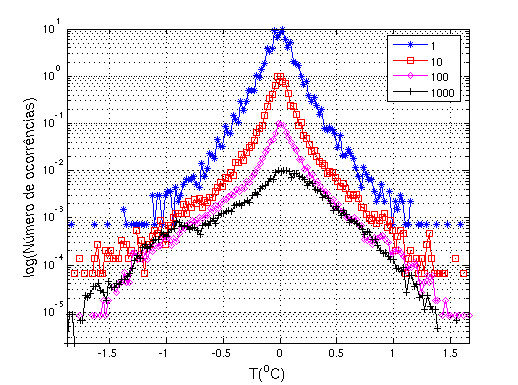
\includegraphics{Figuras2/tS0681200inter.png}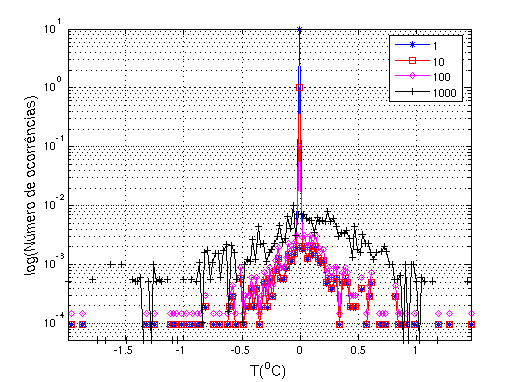
\includegraphics{Figuras2/ctS0681200inter.png}}\\ \resizebox{7.5cm}{!}{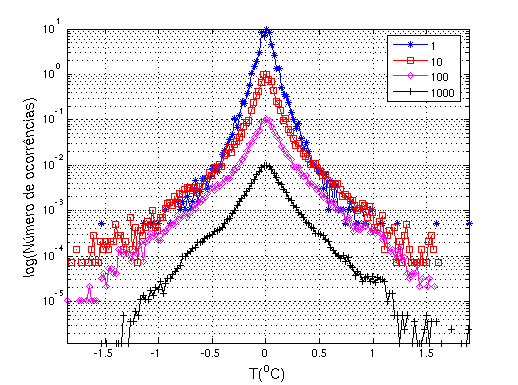
\includegraphics{Figuras2/itS0681200inter.png}}
\caption{FDP's das diferenças das séries de temperatura total, coerente e incoerente em função de diferentes valores de $\Delta r$, respectivamente. Os valores do eixo horizontal foram normalizados pelo desvio padrão associado à cada série.}
\label{figintermitente}
\end{figure}

Pode-se observar que as FDP's são aproximadamente gaussianas apenas nas maiores escalas do escoamento (com valores de curtose próximos de $3$) e fortemente não gaussianas em suas menores escalas, devido ao fenômeno da intermitência. Nas menores escalas de separação, ocorrem grandes flutuações com uma freqüência muito maior que aquela prevista para um processo gaussiano. Este fenômeno, diretamente ligado à intermitência do escoamento turbulento, aparece nas FDP's sob a forma de ``asas'' ou ``caudas'' prolongadas. Pode-se também observar que as FDP's associadas à série coerente são bastante diferentes daquelas associadas às séries total e incoerente. Isto porquê a intermitência presente na série coerente está associada aos maiores vórtices do escoamento (grandes escalas) e ainda a mesma sofre influência direta das condições de contorno. As FDP's associadas à serie incoerente estão associadas aos menores vórtices do escoamento (pequenas escalas) que possuem atributos universais.

Para melhor compreender a forma das curvas das FDP's e, desta forma, quantificar a presença dos fenômenos intermitentes, foram calculados os valores de curtose %(conforme a Equação~(\ref{eqintermitencia})) 
para cada uma das séries temporais (ver Tabela~\ref{tabcurtose}). Pode-se observar que os valores da curtose, em todos os casos, cresce quando $r\rightarrow 0$. Este fato confirma a presença da intermitência em todas as escalas do escoamento.


\begin{table}[!ht]
\begin{center}
\caption{Valores médios da curtose para as séries de temperatura total, coerente e incoerente e seus respectivos desvios padrões.}
\begin{tabular}{c c c c}
\hline 
\textbf{Escala} & \textbf{Série total} & \textbf{Série coerente} & \textbf{Série incoerente} \\
\hline
$\Delta T_{r_{1}}$ & 11.9420$\pm 0.0113$   & 2162.9$\pm 0.0031$   & 19.9782$\pm 0.0117$     \\
%\hline
$\Delta T_{r_{2}}$ & 20.4177$\pm0.0254$  & 216.3161$\pm 0.1050$   & 19.3235$\pm 0.0271$    \\
%\hline
$\Delta T_{r_{3}}$ & 10.9112$\pm0.0548$ & 21.6603$\pm 0.0305$     & 21.6603$\pm 0.0537$    \\
%\hline
$\Delta T_{r_{4}}$ & 5.1312$\pm0.1050$ & 4.8617$\pm 0.0926$    &  8.5637$\pm 0.0510$    \\
\hline

\end{tabular}
\label{tabcurtose}
\end{center}
\end{table}


\subsection{Fluxos}

Na determinação das características da interação solo-atmosfera é de fundamental importância estimar os fluxos de grandezas, tais como momentum, calor sensível, calor latente, dentre outras. Embora existam numerosos métodos para a estimativa de tais fluxos, o único método de medida direta deles é representado pelo \textit{Método das Covariâncias} (MC)~\cite{arya/88}. 

O MC consiste em calcular as covariâncias entre as flutuações de velocidade vertical do vento $w'$ com as flutuações de uma grandeza $s$ da qual se deseja conhecer o fluxo $F_{s}$, nesse caso o fluxo vertical~\cite{arya/88}. Desta forma, o fluxo vertical $F_{s}$ é calculado de acordo com a seguinte relação:

\begin{equation}
F_{s}=\left<w's'\right>=\frac{1}{T}\sum w's'
\label{eqfluxo}
\end{equation}
onde $\left<\right>$ é o operador média, $T$ é a escala utilizada para se realizar a média.

A Figura~\ref{figfluxo} mostra o fluxo turbulento de calor calculado a partir das flutuações associadas às séries de temperatura (tS1200) e velocidade vertical do vento (wS1200) medidas no nível superior da copa e às $12$ horas, com escala de $T=120$. Os picos associados ao fluxo podem tanto corresponder à simultânea elevação de temperatura e velocidade do vento ou à queda simultânea de ambas as grandezas. Os retângulos em vermelho correspondem à ejeção do fluxo enquanto que o retângulo em azul corresponde à queda do fluxo.

Pode-se observar que a presença das estruturas coerentes em rampa, na série tS1200, ocasiona diversos picos no fluxo associado. Este fato ilustra o importante papel que as estruturas coerentes desempenham no transporte de calor (e outras grandezas) através da copa. %, conforme já discutido na Seção~\ref{secturb}.

\begin{figure}[ht]
\centering \resizebox{13cm}{!}{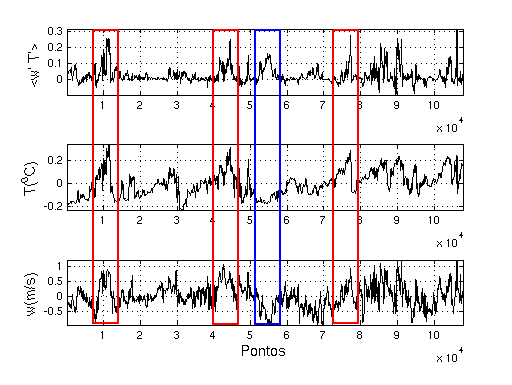
\includegraphics{Figuras2/fluxo.png}}
\caption{Fluxo turbulento de calor associado às flutuações de tS1200 e wS1200. Os retângulos em vermelho delimitam regiões nas quais há uma ejeção do fluxo, enquanto que o retângulo em azul delimita uma região na qual há queda do fluxo.}
\label{figfluxo}
\end{figure}

\section{Investigando a presença de comportamento caótico acima da copa da floresta Amazônica}

%Conforme o Capítulo~\ref{caputiltecnicas}, o espectro de potência, a função de correlação integral, e o maior expoente de Lyapunov fornecem uma orientação para verificar a existência de uma dinâmica caótica em séries temporais experimentais. 

Pode-se observar pela Figura~\ref{figespectrotS0681200} que os espectros de potência para as séries total, coerente e incoerente apresentam um aspecto de ``banda-larga'' e, ainda, que os mesmos não exibem nenhuma freqüência dominante. Assim, tais séries podem estar relacionadas à um sistema dinâmico caótico. Contudo, a caracterização de comportamento caótico em séries temporais, apenas com base no espectro de potência associado, é insuficiente~\cite{tufillaro/92}. 

\subsection{Reconstrução do espaço de estado}

%\paragraph*{A escolha do passo}
\subsubsection{A escolha do passo}
A Figura~\ref{figautocorrtS0681200} mostra a função de autocorrelação, estimada a partir da Equação,%~(\ref{eqautocorr}), 
para as séries total, coerente e incoerente. O primeiro zero desta função para série total corresponde a $\tau=7391\approx 123s$, para a série coerente corresponde a $\tau=8057\approx 134s$, e para a série incoerente corresponde a $\tau=70\approx 1s$. O valor do atraso $\tau$ correspondente a $1/20$ do primeiro zero do valor da função de autocorrelação foi a escolha adotada para a reconstrução do espaço de fase para cada uma das séries, conforme~\citeonline{gallego/01}. Desta forma, os valores $\tau=369$, $\tau=402$ e $\tau=3$ associados às séries total, coerente e incoerente, respectivamente, serão substituídos na relação%~(\ref{eqtakensreconst}), 
e assim será realizada a reconstrução das trajetórias associadas à cada série. 

\begin{figure}[ht]
\centering \resizebox{15cm}{!}{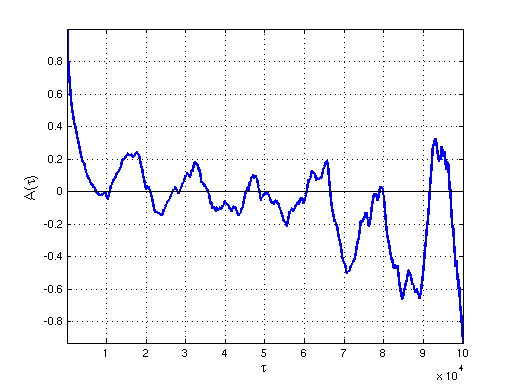
\includegraphics{Figuras2/tS0681200autocorr.png}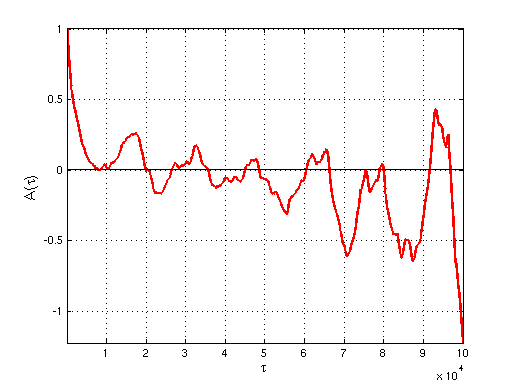
\includegraphics{Figuras/ctS0681200autocorr.png}}\\ \resizebox{7.5cm}{!}{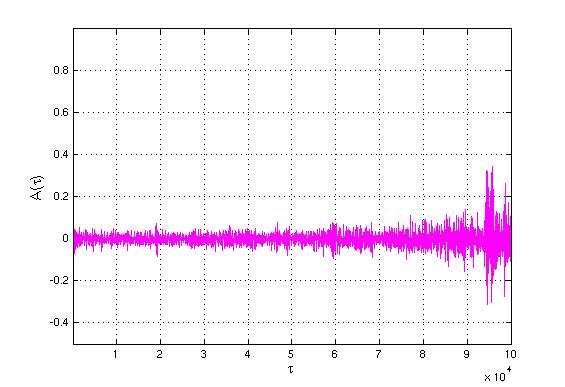
\includegraphics{Figuras2/itS0681200autocorr.png}}
\caption{Função de autocorrelação da série temporal total (em azul), da série temporal coerente (em vermelho) e da série temporal incoerente (em rosa), respectivamente. Tanto para a série total quanto para a série coerente o valor de $A(\tau)$ diminui com o incremento de $\tau$. Para a série incoerente o valor de $A(\tau)$ alterna entre valores positivos e negativos com o incremento de $\tau$.}
\label{figautocorrtS0681200}
\end{figure}

Pode-se observar que a função de autocorrelação $A(\tau)$ tanto para a série total quanto para a série coerente são bastante semelhantes. Para ambos os casos o valor de $A(\tau)$ diminuiu com o incremento de $\tau$ e desta forma, tais séries podem estar relacionadas a um sistema dinâmico com comportamento caótico. O valor de $A(\tau)$ para série incoerente alterna entre valores positivos e negativos com o incremento de $\tau$, e desta forma tal série pode estar associada a algum tipo de aleatoriedade. Porém, como se sabe que a função de autocorrelação não permite, por si só, a caracterização de uma dinâmica caótica determinística, faz-se necessário aplicar outras ferramentas para a caracterização dessa dinâmica nas séries em estudo.

%\paragraph*{A dimensão de imersão}
\subsubsection{A dimensão de imersão}

Após as estimativas dos tempos de atraso $\tau$, as reconstruções dos espaços de fase, a partir de cada uma das séries foram realizadas utilizando a Equação%~(\ref{eqtakensreconst}). 
Desta forma, foi possível calcular a função de correlação integral%~(\ref{eqcorr1}) 
entre os pares de pontos reconstruídos. As dimensões de imersão usadas para as pseudo-fases variam de $1$ a $10$. 

As Figuras~\ref{figcorrinttS0681200} mostram as correlações integrais das séries temporais total, coerente e incoerente versus a escala $r$ em diferentes dimensões de imersão. Pode-se observar que cada uma destas curvas (em escala $\log$-$\log$) possue seções lineares cujos valores das inclinações, calculados via regressão linear, saturam ou não quando as dimensões de imersão são incrementadas. Estes valores de inclinações em função das dimensões de imersão (que é por definição a dimensão de correlação, $D_{2}$) podem ser vistos através da Figura~\ref{figdimcorreltcitS0681200} para cada uma das séries em estudo. Nesta figura pode ser observada também a dimensão de correlação obtida de um processo puramente estocástico (ruído branco). Tanto para a série total quanto para a série coerente a dimensão de correlação satura em aproximadamente $D_{2}=3.5$ e $D_{2}=3.2$, respectivamente com o incremento da dimensão de imersão. Foram feitas $5$ realizações análogas à descrita acima, e a dimensão de correlação média, para a série total, foi de $D_{2}=\langle3.50\rangle$ com desvio padrão de $\sigma_{D_{2}}=0.05$. Para a série coerente, a dimensão de correlação média foi de $D_{2}=\langle3.21\rangle$ com desvio padrão de $\sigma_{D_{2}}=0.04$. Este comportamento sugere fortemente a existência de uma dinâmica caótica de baixa dimensão em tais séries. Já para o sinal incoerente não há saturação, o que descarta a existência de uma dinâmica caótica de baixa dimensão.


\begin{figure}[ht]
\centering \resizebox{15cm}{!}{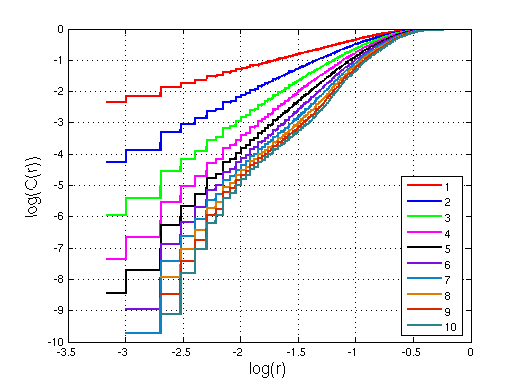
\includegraphics{Figuras2/tS0681200corrint.png}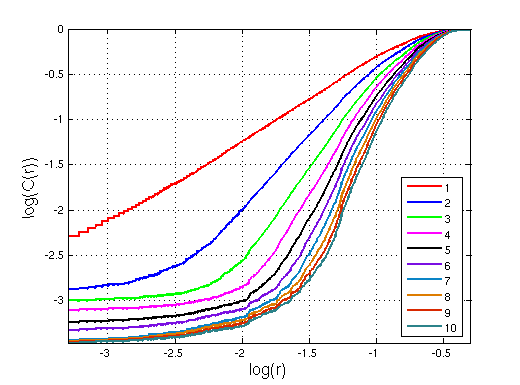
\includegraphics{Figuras/ctS0681200corrint.png}}\\ \resizebox{7.5cm}{!}{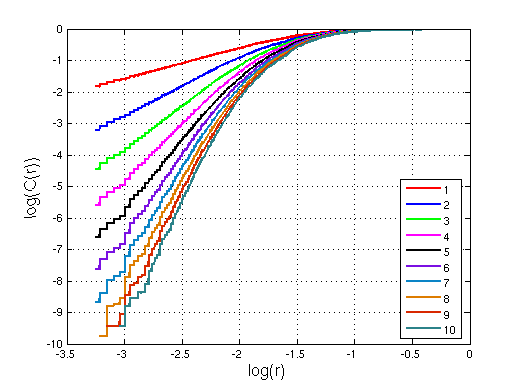
\includegraphics{Figuras/itS0681200corrint.png}}
\caption{Função de correlação integral da série temporal total, da série temporal coerente e da série temporal incoerente, respectivamente.}
\label{figcorrinttS0681200}
\end{figure}

\begin{figure}[ht]
\centering \resizebox{11cm}{!}{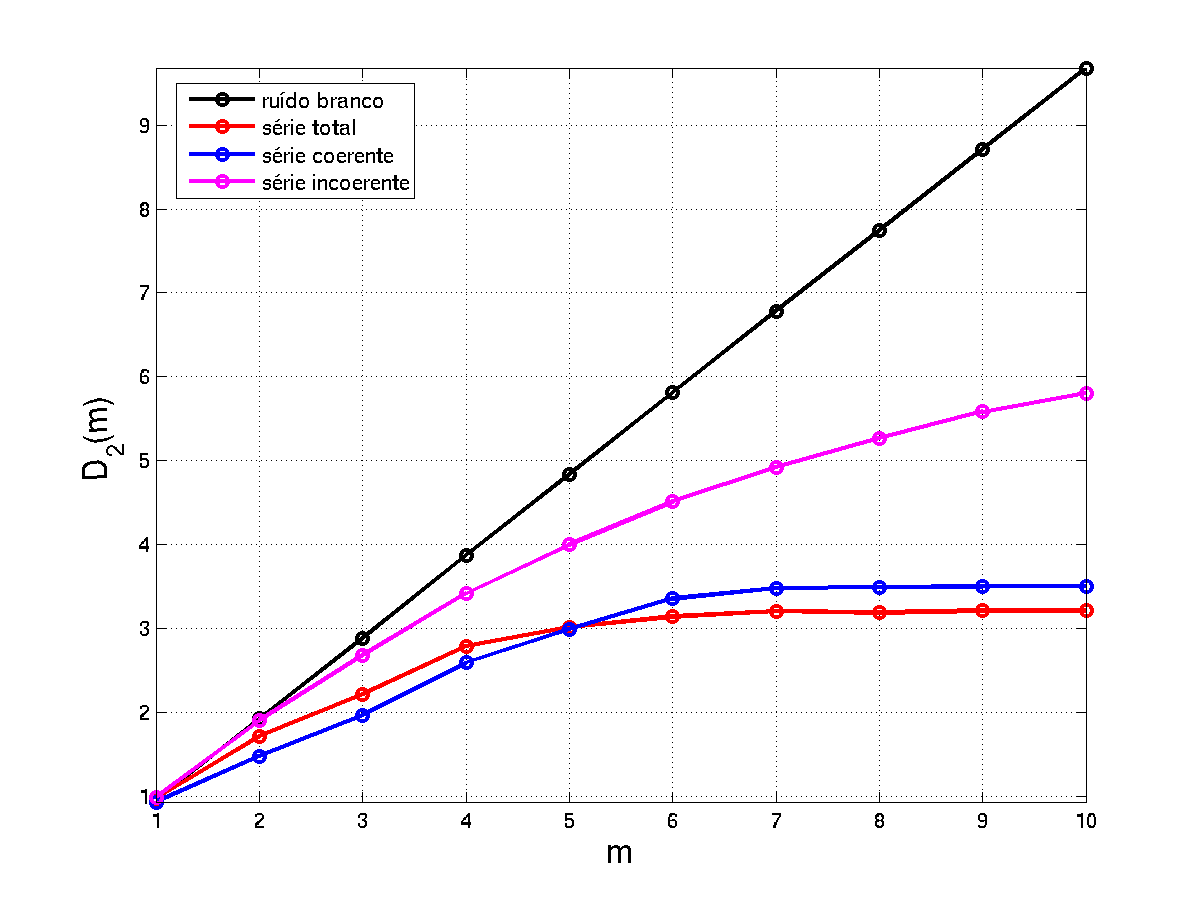
\includegraphics{Figuras2/citS0681200dimcorrel3.png}}
\caption{Dimensão de correlação das séries total, coerente e incoerente, respectivamente. Asteriscos representam uma série aleatória (ruído branco) cuja dimensão de correlação não satura.}
\label{figdimcorreltcitS0681200}
\end{figure}

De acordo com a relação de Takens, %dada por~(\ref{eqconditak}), 
os atratores associados às séries total e coerente podem ser bem representados em espaços de imersão $m=8$. Porém, os valores obtidos para $m$ inviabilizam a visualização dos atratores reconstruídos nesses espaços. Para efeito de ilustração, a Figura~\ref{figatratortS0681200} mostra o atrator associado à série total, imerso no espaço de fase tridimensional. Pode-se observar que a estrutura deste atrator não é totalmente revelada. Isto porque a dimensão do espaço de imersão utilizada é insuficiente.

\begin{figure}[ht]
\centering\resizebox{11cm}{!}{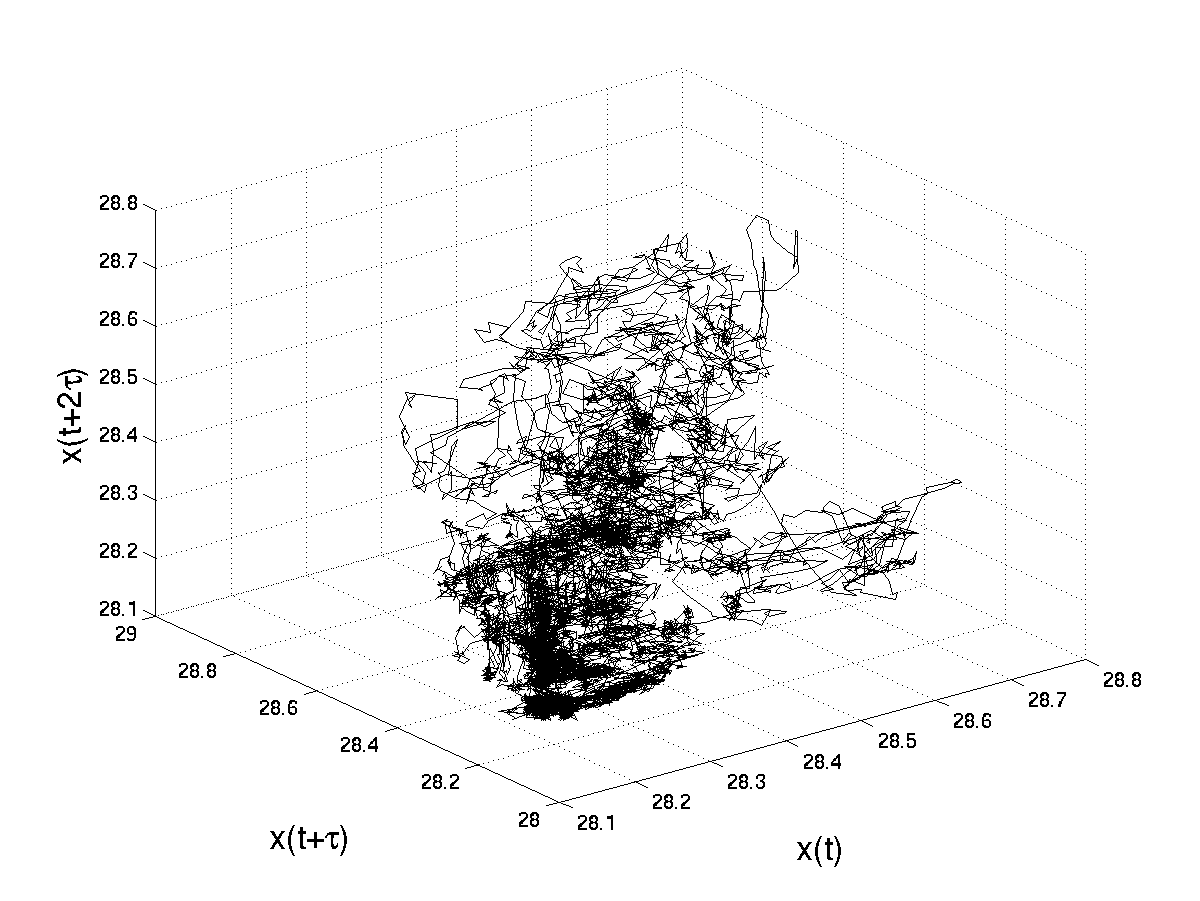
\includegraphics{Figuras2/atratortS0681200.png}}
\caption{Imersão tridimensional do atrator associado à série total com $m=8$ e $\tau=369$.}
\label{figatratortS0681200}
\end{figure}


Os valores obtidos para $D_{2}$ são consistentes com diversos trabalhos que detectaram a presença de atratores caóticos de baixa dimensão com base em dados atmosféricos (ver Tabela~\ref{tabeladimensao}).

\begin{table}[!ht]
\begin{center}
\caption{Valores da dimensão de correlação com base em diversas séries temporais turbulentas.}
%\footnotesize
\small
\begin{tabular}{l l l}
\hline 
\multicolumn{1}{c}{\textbf{Tipo de dado}} & \multicolumn{1}{c}{\boldmath{$D_{2}$}} &  \multicolumn{1}{c}{\textbf{Referência}} \\
\hline
Temperatura (série total)  &   3.50    &  Este trabalho  \\
%\hline
Temperatura (série coerente)  &   3.21   &  Este trabalho  \\
%\hline
Temperatura   &   4.50  &  \citeonline{jaramillo/93}   \\
%\hline
Velocidade do vento (longitudinal)  &   3.50   &   \citeonline{jaramillo/93}  \\
%\hline
Temperatura   &   3.26   &  \citeonline{xin/01} \\
%\hline
Velocidade do vento (longitudinal)   &   3.43   &  \citeonline{xin/01}   \\
%\hline
Velocidade do vento (vertical)   &   5.35  &   \citeonline{gallego/01} \\
\hline
\end{tabular}
\label{tabeladimensao}
\end{center}
\end{table}


É importante observar ainda que a lei dos $-5/3$ de Kolmogorov implica, para um processo estocástico com uma lei de potência no espectro, uma dimensão de correlação de $D_{2}=3$, conforme~\citeonline{osboproven/89}. Como todos os valores para as dimensões de correlações encontradas estão acima de $D_{2}=3$, pode-se concluir que as séries temporais total e coerente não podem ser representadas por um processo puramente estocástico, o que já era esperado.

Em seguida, foram realizados os ``testes surrogate'', conforme~\citeonline{provenzalesmith/92} para a série total e coerente. Desta forma, foram obtidas duas novas séries temporais a partir do embaralhamento das fases das séries originais. As reconstruções dos espaços de fase, a partir de cada uma das novas séries foram realizadas utilizando novamente a Equação,%~(\ref{eqtakensreconst}), 
com os mesmos atrasos temporais utilizados anteriormente. A Figura~\ref{figtS0681200surr}(a) mostra a correlação integral da série temporal obtida do surrogate da série total, enquanto que a Figura~\ref{figtS0681200surr}(b) mostra a correlação integral da série temporal obtida do surrogate da série coerente (ambas em dimensões de imersão que variam de $1$ a $10$). A Figura~\ref{figtS0681200surr}(c) apresenta a dimensão de correlação obtida para o surrogate de cada uma das séries. Foram feitas $5$ realizações análogas à descrita acima, e pôde-se observar que a dimensão de correlação $D_{2}$ em todos os casos não satura. Esse comportamento sugere fortemente a existência de uma dinâmica de baixa dimensão em tais séries temporais~\cite{provenzalesmith/92}.

\begin{figure}[ht]
\centering \resizebox{15cm}{!}{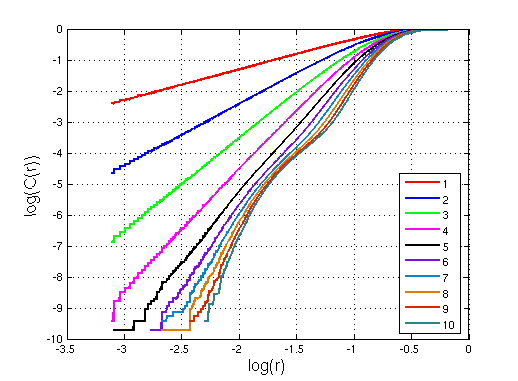
\includegraphics{Figuras2/tS0681200surrcorrelint.png}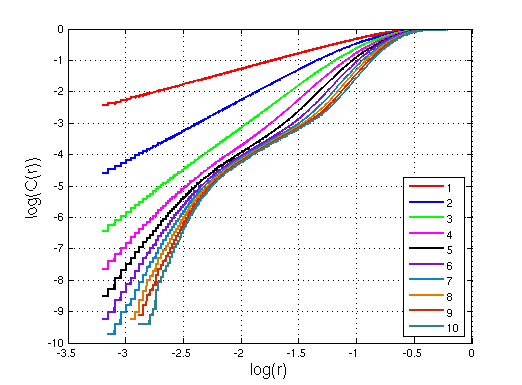
\includegraphics{Figuras/ctS0681200surrcorrelint.png}}\\ \resizebox{7.5cm}{!}{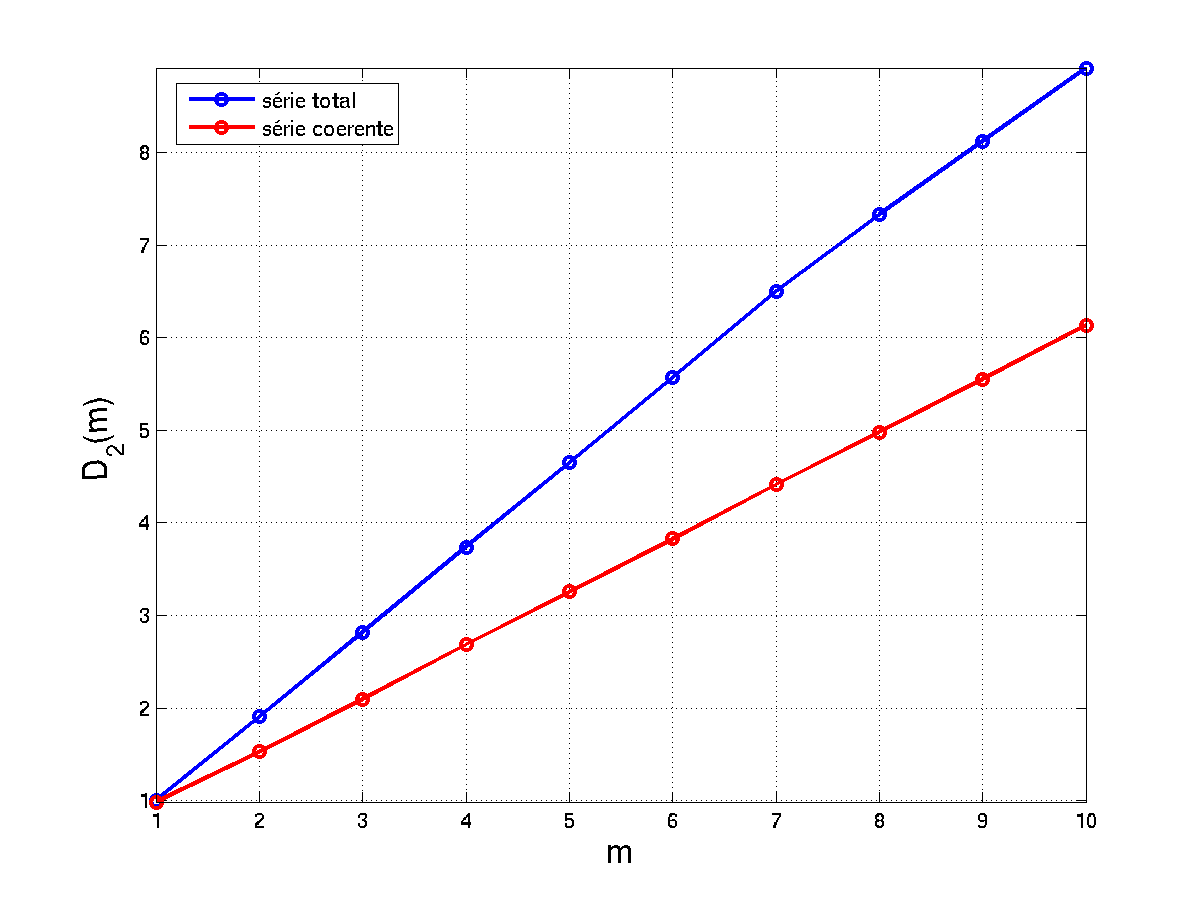
\includegraphics{Figuras/tecS0681200dimcorrsurr2.png}}
\caption{(a) Correlação integral do surrogate associado à série total com $m=1$ a $10$. (b) Correlação integral do surrogate associado à série coerente com $m=1$ a $10$. (c) Dimensões de correlação associadas ao surrogate das séries total e coerente.}
\label{figtS0681200surr}
\end{figure}

Outro teste considerado foi a análise da correlação integral da primeira derivada numérica conforme~\citeonline{provenzalesmith/92} da série temporal total e coerente. Desta forma, foram obtidas duas novas séries temporais a partir das séries anteriores. As reconstruções dos espaços de fase, a partir de cada uma das novas séries foram realizadas utilizando novamente a Equação,%~(\ref{eqtakensreconst}), 
agora com atrasos temporais de $\tau=2$ e $\tau=3$, respectivamente. A Figura~\ref{figtS0681200diff}(a) apresenta a correlação integral da série temporal obtida a partir da primeira derivada numérica associada à série total e (b) apresenta a correlação integral da série temporal obtida a partir da primeira derivada numérica associada à série coerente. Pode-se observar que em ambos os casos, os valores da correlação integral para $m=1$ a $10$ apresentam-se concentrados em poucos valores $r$ e ainda tais valores variam bruscamente com o incremento de $r$. Isto ocorre porquê os valores assumidos pelas séries temporais total e coerente apresentam poucas variações da média e, conseqüentemente, as primeiras derivadas associadas possuem um número expressivo de valores próximos de zero ou nulos. Tal fato inviabiliza estimativa da correlação integral e, conseqüentemente, de $D_{2}$. Desta forma, este teste foi descartado das análises associadas à dinâmica de baixa dimensão associadas às séries total e coerente.

\begin{figure}[ht]
\centering \resizebox{15cm}{!}{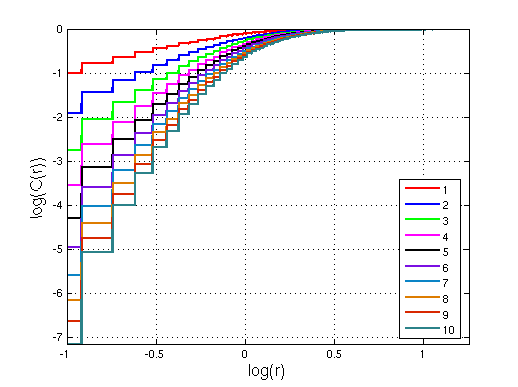
\includegraphics{Figuras2/tS0681200corrintdiff.png}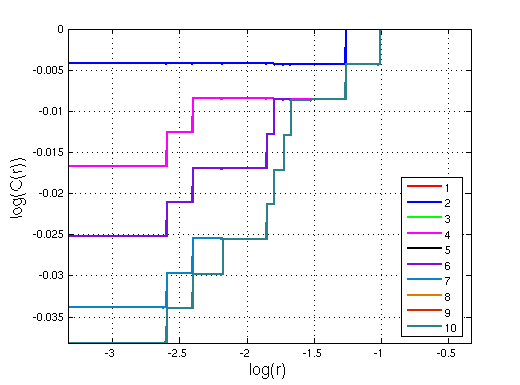
\includegraphics{Figuras/ctS0681200corrintdiff.png}}\\ 
\caption{(a) Correlação integral da primeira derivada associada à série total com $m=1$ a $10$. (b) Correlação integral da primeira derivada associada à série coerente com $m=1$ a $10$.}
\label{figtS0681200diff}
\end{figure}

Pode-se ainda observar que os valores de $D_{2}$ associados às séries total e coerente, com base em $108.000$ pontos em ambas as séries, é confiável já que seus valores dados respectivamente por $D_{2}=3.50$ e $D_{2}=3.21$, satisfazem a relação%~(\ref{eqlimitemax}) 
conforme~\citeonline{eckruelllyap/92}.

%\paragraph*{Expoentes de Lyapunov}
\subsubsection{Expoentes de Lyapunov}

Após a estimativa da dimensão de imersão, foi possível realizar as reconstruções dos atratores associados às séries temporais total e coerente em espaços de fase adequados. Desta forma, foi possível obter, com base no algoritmo de \citeonline{wolf/85}, aproximações numéricas dos maiores expoentes de Lyapunov associados às séries total e coerente. A Figura~\ref{figtS0681200lyap} mostra as evoluções no tempo de tais expoentes. O cálculo do maior expoente de Lyapunov foi realizado em diferentes regiões dos atratores associados, e desta forma, os valores médios obtidos foram de $\lambda_{1}=0.050\pm0.002$ para a série total e de $\lambda_{1}=0.011\pm0.001$ para a série coerente. Pode-se observar que valor de $\lambda_{1}$ é estritamente positivo em ambos os casos, o que sugere a presença da dinâmica caótica em ambas as séries. 
 
\begin{figure}[ht]
\centering \resizebox{15cm}{!}{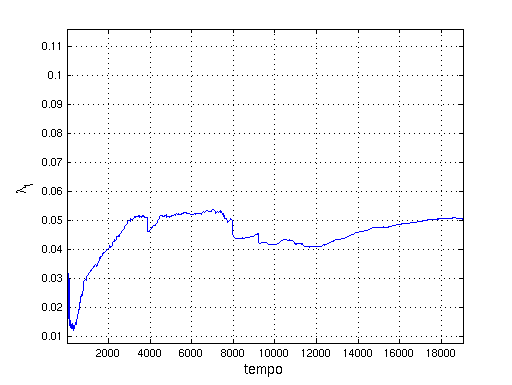
\includegraphics{Figuras2/tS0681200lyapcorr.png}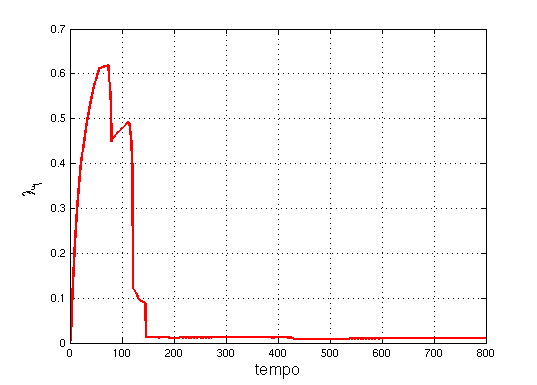
\includegraphics{Figuras/coertS0681200lyaptak.png}}
\caption{(a) Convergência do maior expoente de Lyapunov ($\lambda_1$) associado à série temporal total. (b) Convergência do maior expoente de Lyapunov ($\lambda_1$) associado à série temporal coerente.}
\label{figtS0681200lyap}
\end{figure}

Os valores obtidos para o expoente de Lyapunov $\lambda_{1}$ são consistentes com diversos trabalhos que detectaram a presença de atratores de baixa dimensão com base em dados atmosféricos (ver Tabela~\ref{tabelalyapunov}).

\begin{table}[!ht]
\begin{center}
\caption{Valores dos expoentes de Lyapunov com base em diversas séries temporais turbulentas.}
%\footnotesize
\small
\begin{tabular}{l l l}
\hline 
\multicolumn{1}{c}{\textbf{Tipo de dado}} & \multicolumn{1}{c}{\boldmath{$\lambda_{1}$}} & \multicolumn{1}{c}{\textbf{Referência}} \\
\hline
Temperatura (série total)  &  0.050   &  Este trabalho  \\
%\hline
Temperatura (série coerente)  &  0.011    &  Este trabalho  \\
%\hline
Temperatura   &  0.155  &  \citeonline{jaramillo/93}   \\
%\hline
Velocidade do vento (longitudinal)  &  0.195   &   \citeonline{jaramillo/93}  \\
%\hline
Temperatura  &  0.047   &  \citeonline{xin/01} \\
%\hline
Velocidade do vento (vertical) &  0.067    &  \citeonline{gallego/01}   \\
%\hline
Velocidade do vento (vertical)  &   0.058  &   \citeonline{gallego/01} \\
\hline
\end{tabular}
\label{tabelalyapunov}
\end{center}
\end{table}

%\paragraph*{Plots de recorrência}
\subsubsection{Plots de recorrência}

A técnica dos PRs foi aplicada nas séries total, coerente e incoerente. Como o número de pontos em todas as séries é muito grande ($108.000$ pontos) foi necessário reduzir o número de pontos em cada caso. A estratégia adotada foi construir novas séries temporais, com $10.800$ pontos, através de janelas de dados deslizantes de $10$ pontos. Desta forma, os valores obtidos para as novas séries correspondem seqüencialmente a médias de $10$ valores das séries antigas.

A Figura~\ref{figrptemps} apresenta PRs para às séries total, coerente e incoerente. Pode-se observar que os PRs associados às séries total e coerente possuem estruturas diagonais paralelas à diagonal principal, conforme Figura~\ref{figrptemps}(a) e (b). Essas estruturas ocorrem quando um segmento da trajetória reconstruída é paralelo à outro segmento, ou seja, a trajetória visita a mesma região do espaço de fase em diferentes tempos. Sabe-se que a repetição de estados é uma propriedade fundamental de um sistema dinâmico determinístico, e é um comportamento típico em sistemas caóticos ou não-lineares~\cite{thieltese/04}. Desta forma, a tanto a série temporal total quanto a série coerente podem estar associadas à um sistema dinâmico determinístico caótico. Porém, o PR associado à série incoerente apresenta um padrão bem distinto quando comparado aos obtidos para a série total e coerente. O PR associado a esta série apresenta uma homogeneidade em relação à distribuição de seus pontos, conforme Figura~\ref{figrptemps}(c), que é um comportamento típico de sistemas estocásticos~\cite{thieltese/04}. 
%ver papers dos plots de recorrencia!!!
\begin{figure}[ht]
\centering 
\resizebox{7.2cm}{!}{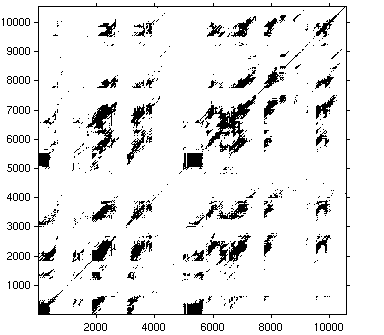
\includegraphics{Figuras2/tS0681200rp.png}} \resizebox{7.2cm}{!}{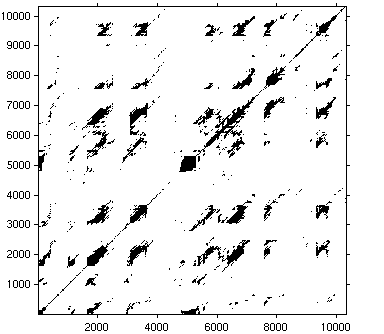
\includegraphics{Figuras2/ctS0681200rp.png}} \\  \resizebox{7.2cm}{!}{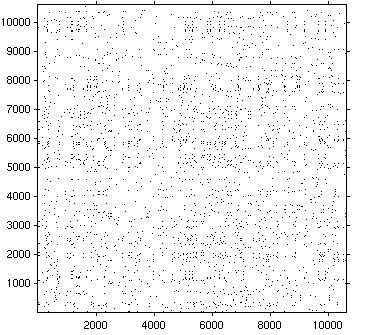
\includegraphics{Figuras2/itS0681200rp.png}} 
\caption{(a) PR associado à série total com $m=8$ e $\varepsilon=0.9507$ . (b) PR associado à série coerente $m=8$ e $\varepsilon=0.8390$. (c) PR associado à série incoerente $m=1$ e $\varepsilon=0.030$. Os valores de $\varepsilon$ utilizados nos casos (a) e (b) correspondem à $10\%$ do diâmetro do espaço de fase~\cite{thielromano/04}, já no caso (c) corresponde à $10\%$ da variância associada.}
\label{figrptemps}
\end{figure}


\section{Investigando a presença de comportamento caótico abaixo da copa da floresta Amazônica}

Nesta seção será investigada a possível natureza caótica de duas outras séries temporais de temperatura, a saber, tM1200 e tI1200, sendo que as mesmas não possuem estruturas coerentes do tipo rampa, conforme~Figura~\ref{figseriestempdiur}. Se a dinâmica de baixa dimensão obtida nas análises precedentes, com base na série temporal tS1200, está associada exclusivamente à existência das estruturas coerentes, espera-se que as séries de temperatura tM1200 e tI1200 não estejam associadas a um sistema de baixa dimensão.

\subsection{Espectros de potência}

Os espectros de potência das séries temporais de temperatura medidas nos níveis médio e inferior da copa às $12$ horas (tM1200 e tI1200) foram estimados usando FFT. Resultados mostram que a inclinação desses espectros (em escala $\log$-$\log$) coincidem com a lei dos $-5/3$ de Kolmogorov em ambas as séries. 

A Figura~\ref{figespectrotMI0681200} apresenta os espectros de potência para cada uma das séries, calculados pela relação.%~(\ref{eqespectrodiscr}). 
Pode-se observar um aspecto de ``banda-larga'' em ambos os espectros e que os mesmos não exibem nenhuma freqüência dominante. Assim, o comportamento caótico nas séries não pode ser excluído de análises posteriores.


\begin{figure}[ht]
\centering \resizebox{15cm}{!}{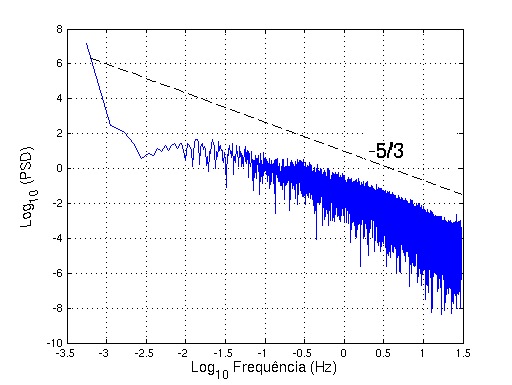
\includegraphics{Figuras2/tM0681200espectro.png}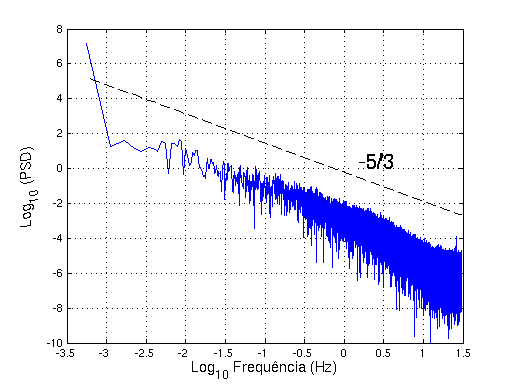
\includegraphics{Figuras2/tI0681200espectro.png}}
\caption{Espectros de potência das séries temporais tM1200 e tI1200, respectivamente. Observe que as inclinações destes espectros no SI (em escala $\log$-$\log$) coincidem com a lei dos $-5/3$ de Kolmogorov}
\label{figespectrotMI0681200}
\end{figure}

\subsection{Reconstrução do espaço de estado}

%\paragraph*{A escolha do passo}
\subsubsection{A escolha do passo}
Os tempos de atraso $\tau$ para as séries tM1200 e tI1200 foram estimados. %a partir da Equação ~(\ref{eqautocorr}). 
A Figura~\ref{figautocorrtMI0681200} mostra a função de autocorrelação para cada uma das séries. O primeiro zero desta função para a primeira série corresponde a $\tau=13.020\approx217s$ e para a segunda série corresponde a $\tau=3.205\approx 53s$. Desta forma, os valores $\tau=651$ e $\tau=160$ associados às séries tM1200 e tI1200, respectivamente, serão substituídos na relação %(\ref{eqtakensreconst}), 
e assim será realizada a reconstrução das trajetórias associadas à cada série.  


\begin{figure}[ht]
\centering \resizebox{15cm}{!}{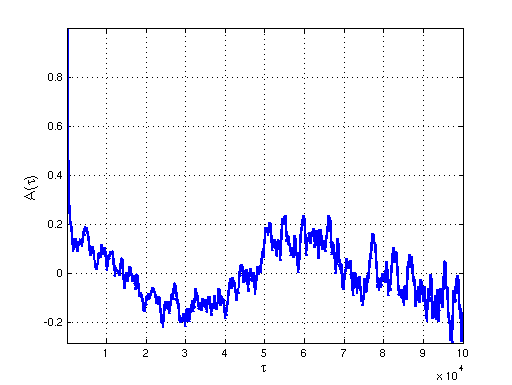
\includegraphics{Figuras2/tM0681200autocorr.png}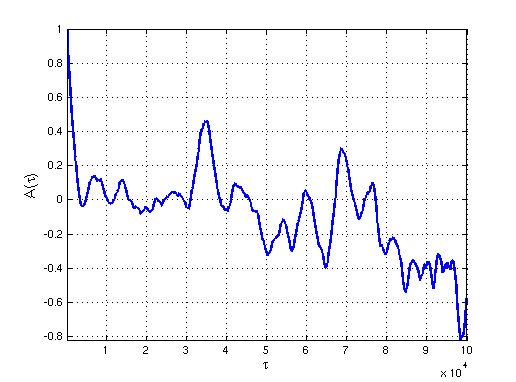
\includegraphics{Figuras2/tI0681200autocorr.png}}
\caption{Função de autocorrelação das séries temporais tM1200 e tI1200, respectivamente. Os valores de $A(\tau)$ em ambos os casos diminui com o incremento de $\tau$, }
\label{figautocorrtMI0681200}
\end{figure}

Pode-se observar que a função de autocorrelação $A(\tau)$ em ambos os casos diminui com o tempo (ou equivalentemente com o incremento de $\tau$) e, desta forma, tais séries podem estar relacionadas a um sistema dinâmico com comportamento caótico. Entretanto, faz-se necessário aplicar outras ferramentas de detecção de comportamento caótico nas séries em estudo.

%\paragraph*{A dimensão de imersão}
\subsubsection{A dimensão de imersão}

Após as estimativas dos tempos de atraso $\tau$, as reconstruções dos espaços de fase, para as séries temporais tM1200 e tI1200 foram realizadas utilizando a Equação%~(\ref{eqtakensreconst}). 
Desta forma, foi possível calcular a função de correlação integral%~(\ref{eqcorr1}) 
entre os pares de pontos reconstruídos. As dimensões de imersão usadas para as pseudo-fases variam de $1$ a $10$. 

A Figura~\ref{figcorrintMI0681200} mostra as correlações integrais das séries temporais tM1200 e tI1200 versus a escala $r$ em diferentes dimensões de imersão. Os valores das inclinações (em escalas $\log$-$\log$) das seções lineares associados à cada curva podem ser vistos através da Figura~\ref{figdimcorreltMI0681200} para ambas as séries. Nesta figura pode ser observada também a dimensão de correlação obtida de um processo puramente estocástico (ruído branco). Tanto para a série tM1200 quanto para a série tM1200 não há saturação da dimensão de correlação, o que descarta a existência de uma dinâmica caótica de baixa dimensão em tais séries. 

\begin{figure}[ht]
\centering \resizebox{15cm}{!}{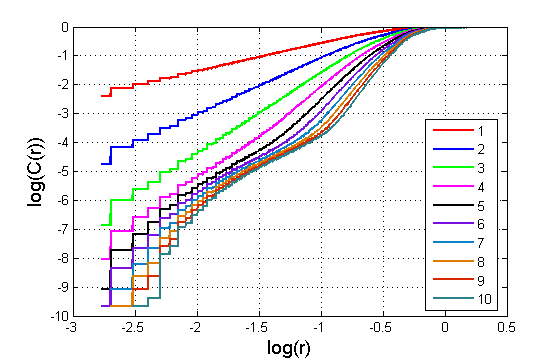
\includegraphics{Figuras2/tM0681200correlint.png}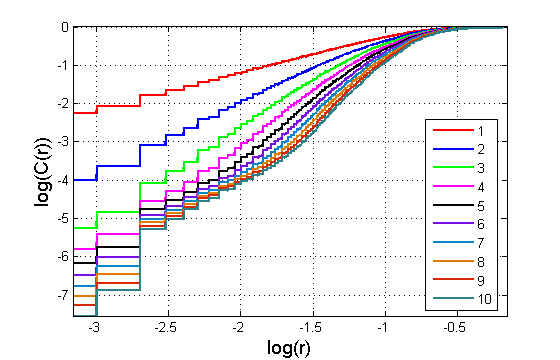
\includegraphics{Figuras2/tI0681200correlint.png}}
\caption{Função de correlação integral das séries temporais tM1200 e tI1200, respectivamente. As dimensões de imersão usadas para as pseudo-fases variam de $1$ a $10$.}
\label{figcorrintMI0681200}
\end{figure}


\begin{figure}[ht]
\centering \resizebox{11cm}{!}{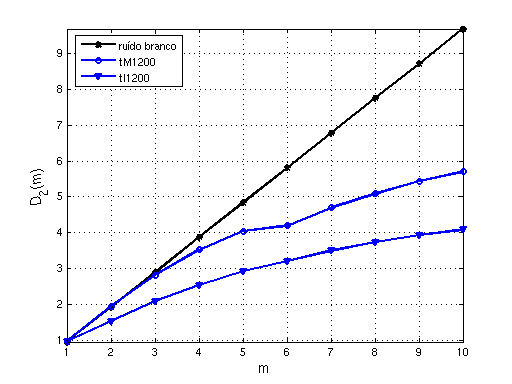
\includegraphics{Figuras2/tMI0681200dimcorrel.png}}
\caption{Dimensões de correlação das séries tM1200 e tI1200. Asteriscos representam uma série aleatória (ruído branco).}
\label{figdimcorreltMI0681200}
\end{figure}

Uma das possíveis justificativas para a não saturação da dimensão de correlação em tM1200 e tI1200 é a ausência de estruturas coerentes do tipo rampa. Porém, pôde-se observar que o espectro de potências das séries tS1200, tM1200 e tI1200 as caracterizam como turbulentas, conforme Figuras~\ref{figespectrotS0681200} e \ref{figespectrotMI0681200}. Desta forma, a detecção experimental de uma dinâmica caótica de baixa dimensão (conforme constatado em tS1200) pode não estar relacionada ao fenômeno da turbulência ``per se'', mas pela existência de estruturas coerentes na atmosfera, como de certa forma intuído por \citeonline{loratrat/91}.